\documentclass[]{beamer}
%for printing or having a crappy pdf reader backup
%\documentclass[handout]{beamer}
\mode<presentation>
\usetheme{Madrid}


\usecolortheme[RGB={80,0,0}]{structure}
%teal \usecolortheme[RGB={0,128,128}]{structure}
\useoutertheme{miniframes}
\useinnertheme{default}
\usepackage{color}
\definecolor{Maroon}{RGB}{80,0,0}
\definecolor{BurntOrange}{RGB}{204,85,0}
\usepackage{setspace}
\usepackage{amsmath}
\usepackage{amsthm}
\usepackage{amsfonts}
\usepackage{amssymb}
\usepackage{verbatim}
\usepackage{array}
\usepackage{graphicx}
\usepackage{subfigure}
\usepackage{colortbl}
\usepackage[retainorgcmds]{IEEEtrantools}
\usepackage{wrapfig}
\usepackage[figurename=,tablename=]{caption}
\usepackage{multirow}
\setbeamercolor{normal text}{fg=black}
\setbeamercovered{dynamic}
\beamertemplatetransparentcovereddynamicmedium
%\usepackage{chronology}
\setbeamertemplate{caption}[numbered]


\newcommand {\mathsym}[1]{{}}
\newcommand {\unicode}{{}}
\newcommand{\om}{\boldsymbol{\Omega}}
\newcommand{\etal}{{\it et al.\,}}

\newlength \figwidth
\setlength \figwidth {0.5\textwidth}


\begin{document}

\title[DFEM Diffusion]{A DFEM Formulation of the Diffusion Equation on Arbitrary Polyhedral Grids}
\author[Hackemack and Ragusa]{Michael Hackemack \& Jean Ragusa \\ {\scriptsize mike\_hack@tamu.edu \& jean.ragusa@tamu.edu}}
\institute[TAMU]{Texas A\&M University \\ Department of Nuclear Engineering}
\date[November 7, 2014]
%\date[2013-2-18]{2013-2-18, rev 1: 2013-3-1, rev 2: 2013-3-4, rev 3: 2013-3-6}

{
\setbeamertemplate{headline}[default] 
\begin{frame}
\vspace{-1.5cm}
	\begin{figure}[t]
		\centering
			
\includegraphics[width=.25\textwidth]{images/seal.png}
	\end{figure}
\vspace{-0.75cm}
\titlepage
\end{frame}

}
\begin{frame}
\tableofcontents
\end{frame}

%%%%%%%%%%%%%%%%%%%%%%%%%%%%%%%%%%%%%%%%%%%%%%%%%%%%%%%%%%%%%
%%%%%%%%%%%%%%%%%%%%%%%%%%%%%%%%%%%%%%%%%%%%%%%%%%%%%%%%%%%%%
\section{Problem Description}
\subsection{}
%---------------------------
\begin{frame}[t]\frametitle{Polyhedral Grid Motivation}
         \begin{block}{}{\footnotesize
			\begin{itemize}
				\item Other physics communities are now employing polyhedral grids due to decreased cell/face counts (CFD in particular)
				\item Independently-generated simplicial grids ({\em i.e.} created in parallel) can be stitched together with polyhedra without communicating the whole mesh across processors
				\item Hanging nodes from non-conforming meshes are not necessary (arise naturally in adaptive mesh refinement)
			\end{itemize}}
         \end{block}
	\begin{columns}
		\begin{column}{.5\textwidth}
			\begin{figure}[t]
				\centering
				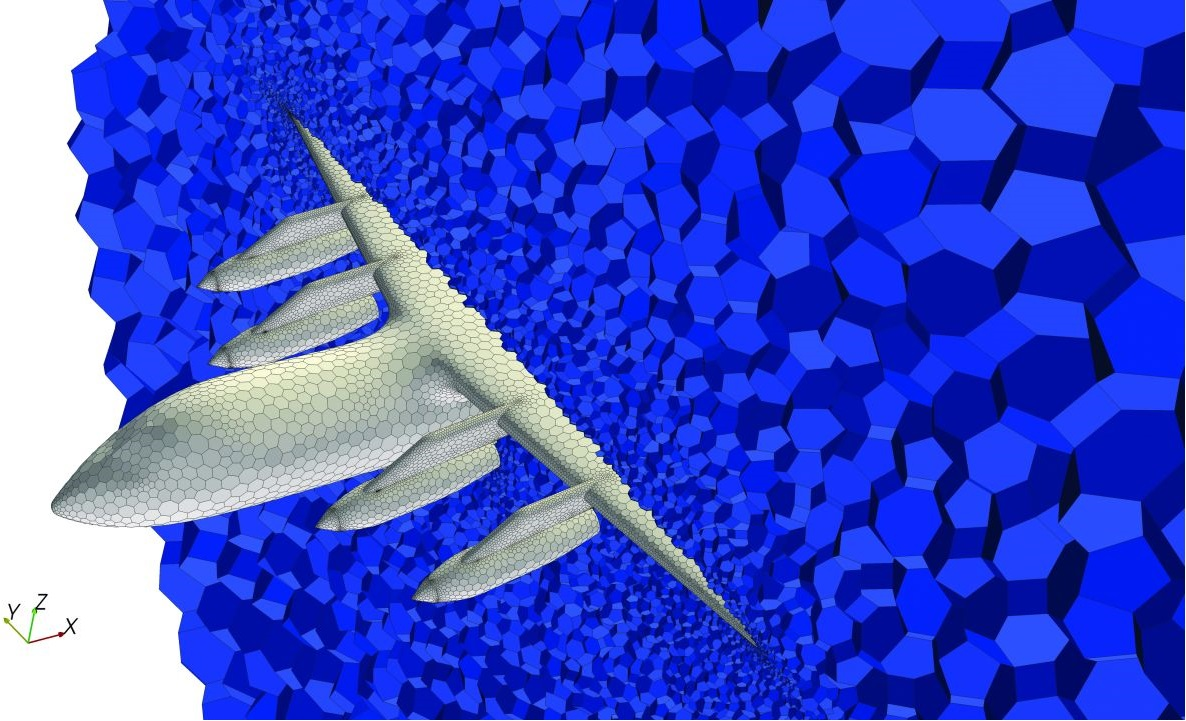
\includegraphics[width=.60\textwidth]{images/Polymesh_sized.jpg} \\
				{\tiny $^{*}$http://www.cd-adapco.com }
			\end{figure}
		\end{column}
		\begin{column}{.5\textwidth}
			\begin{figure}[t]
				\centering
				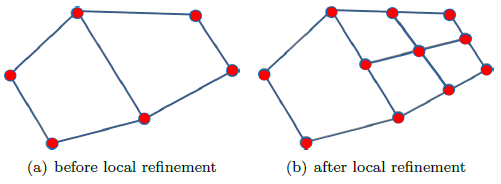
\includegraphics[width=0.85\textwidth]{images/local_refinement.png}
			\end{figure}
		\end{column}
	\end{columns}
\end{frame}
%---------------------------
\begin{frame}[t]\frametitle{Motivation}
{\small
         \begin{block}{}
        	 \begin{itemize}
	      		\item Parallel Deterministic Transport (PDT) code at Texas A\&M to implement transport sweeps on arbitrary grids.
	      		\begin{itemize}{\small
	      			\item Workhourse solution method employs a Discontinuous Finite Element (DFEM) discretization of the transport equation.
	      			\item Code has been tested out to $O(10^6)$ processors
	      		}\end{itemize}
				\item However, convergence issues may arise in thick diffusive configurations
				\begin{itemize}{\small
					\item Need to precondition the transport sweeps
					\item Common to employ Diffusion Synthetic Acceleration (DSA)
				}\end{itemize}
				\item Use same DFEM basis functions as transport equation for DSA
				\begin{itemize}{\small
					\item DSA update has a 1-to-1 mapping on spatial degrees of freedom (DoF)
					\item Eliminates approximate update corrections necessary with Continuous Finite Elements (CFEM) DSA
				}\end{itemize}
		\end{itemize}
         \end{block}
}
\end{frame}
%---------------------------
%%%%%%%%%%%%%%%%%%%%%%%%%%%%%%%%%%%%%%%%%%%%%%%%%%%%%%%%%%%%%
%%%%%%%%%%%%%%%%%%%%%%%%%%%%%%%%%%%%%%%%%%%%%%%%%%%%%%%%%%%%%
\section{DFEM Diffusion Formulation}
\subsection{}
%---------------------------
\begin{frame}[t]\frametitle{The Diffusion Equation}
	\begin{block}{} {\small 
     		\begin{align*}
 	 		{ \small -\vec{\nabla} \cdot D \vec{\nabla} \Phi (\vec{r}) + \sigma \Phi (\vec{r}) = q (\vec{r}), \qquad  \vec{r} \in \mathcal{D} }
        	\end{align*} 
		Dirichlet Boundary Condition:
		\begin{align*}
 	 		{ \small \Phi (\vec{r})  = \Phi_0 (\vec{r})  \qquad \vec{r} \in \partial \mathcal{D}^d }
        	\end{align*} 
		Neumann Boundary Condition:
		\begin{align*}
 	 		{ \small -D \partial_n \Phi (\vec{r})  = J_0 (\vec{r})  \qquad \vec{r} \in \partial \mathcal{D}^n }
        	\end{align*} 
		Robin Boundary Condition:
		\begin{align*}
 	 		{ \small \frac{1}{4} \Phi (\vec{r})  + \frac{1}{2}D \partial_n \Phi (\vec{r})  = J^{inc} (\vec{r})  \qquad \vec{r} \in \partial \mathcal{D}^r}
        	\end{align*} }
    \end{block}
\end{frame}
%---------------------------
\begin{frame}[t]\frametitle{The Diffusion Equation}
	\begin{block}{Weak Form (after divergence theorem)} {\small
		\begin{gather*}
			\Big<  D \vec{\nabla}  \Phi , \vec{\nabla} \Phi^*  \Big>_{\mathcal{D}} - \Big\{    D \partial_n \Phi, \Phi^* \Big\}_{\partial \mathcal{D}} + \Big< \sigma  \Phi ,  \Phi^*  \Big>_{\mathcal{D}} = \Big<q,  \Phi^*  \Big>_{\mathcal{D}}, \qquad \partial_n \equiv \vec{n} \cdot \vec{\nabla}
		\end{gather*}}
	\end{block}
	\begin{block}{Inner Products} {\small
		\begin{gather*}
			\Big<  f , g  \Big>_{\mathcal{D}} \equiv \sum_{K \in \mathcal{T}_h} \int_{K} f  g,  \qquad \Big\{  f , g  \Big\}_{ \mathcal{E}_h} \equiv \sum_{e \in \mathcal{E}_h} \int_{e} f  g
		\end{gather*}
		\begin{gather*}
			\bigcup_{K \in \mathcal{T}_h} K = \mathcal{D},  \qquad \mathcal{E}_h^{\partial \mathcal{D}} =  \mathcal{E}_h^{\partial \mathcal{D}^d} \cup \mathcal{E}_h^{\partial \mathcal{D}^n} \cup \mathcal{E}_h^{\partial \mathcal{D}^r}
		\end{gather*}
	}\end{block}
\end{frame}
%---------------------------
\begin{frame}[t]\frametitle{Penalty Method - Dirichlet Boundaries}
	\begin{block}{Penalty Boundary Term}
		\begin{gather*}
			\Phi (\vec{r}) +\frac{1}{\mu}\partial_n \Phi (\vec{r}) = \Phi_0 (\vec{r}), \qquad \vec{r} \in \partial \mathcal{D}^d, \qquad \mu \gg 1
		\end{gather*}
	\end{block}
	\begin{block}{Laplacian Term}
		\begin{align*}
			\Big<   \vec{\nabla}  \Phi , \vec{\nabla} \Phi^*  \Big>_{\mathcal{D}} - \Big\{    \partial_n \Phi, \Phi^* \Big\}_{\partial \mathcal{D}^d} - \Big\{  \Phi, \partial_n \Phi^* \Big\}_{\partial \mathcal{D}^d} \\ + \Big\{ \mu (\Phi - \Phi_0),  \Phi^* \Big\}_{\partial \mathcal{D}^d} = - \Big\{  \Phi_0, \partial_n \Phi^* \Big\}_{\partial \mathcal{D}^d} 
		\end{align*}
	\end{block}
\end{frame}
%---------------------------
\begin{frame}[t]\frametitle{Interior Penalty Method - Interior Faces}
{\small
	\begin{block}{Interior Faces - Arnold's Extension}
     		\begin{gather*}
			   \Big\{ \mu [\![   \Phi ]\!] , [\![  \Phi^* ]\!]\Big\}_{E_h^i} - \Big\{  [\![   \Phi ]\!] , \{\!\{  D \partial_n \Phi^* \}\!\}\Big\}_{E_h^i} -\Big\{ \{\!\{  D \partial_n  \Phi \}\!\} , [\![  \Phi^* ]\!]\Big\}_{E_h^i} = 0 \\
			 E_h^i = \bigcup_{K_1, K_2 \in \mathcal{T}_h} \left(  \partial K_1  \cap  \partial K_2  \right)
        	\end{gather*}
	\end{block}
	\begin{block}{Mean Value and Jump}
     		\begin{gather*}
			 \{\!\{  \Phi \}\!\} \equiv \frac{\Phi^+ + \Phi^-}{2}, \qquad [\![   \Phi ]\!] \equiv \Phi^+ - \Phi^- 
        	\end{gather*}
		\begin{gather*}
			\Phi^{\pm} \equiv \lim_{s \rightarrow 0^{\pm}} \Phi (\vec{r} + s \vec{n})
        	\end{gather*}
	\end{block}
}
\end{frame}
%---------------------------
\begin{frame}[t]\frametitle{Symmetric Interior Penalty (SIP) Form}
	\begin{block}{Bilinear Form}
		\begin{gather*}
			 a( \Phi, \Phi^*)  = \Big<  D \vec{\nabla}  \Phi , \vec{\nabla} \Phi^*  \Big>_{\mathcal{D}} + \Big<  \sigma   \Phi ,  \Phi^*  \Big>_{\mathcal{D}}    \\
			+  \Big\{ \kappa_e^{SIP} [\![   \Phi ]\!] , [\![  \Phi^* ]\!]\Big\}_{E_h^i} - \Big\{  [\![   \Phi ]\!] , \{\!\{  D \partial_n \Phi^* \}\!\}\Big\}_{E_h^i} -\Big\{ \{\!\{  D \partial_n  \Phi \}\!\} , [\![  \Phi^* ]\!]\Big\}_{E_h^i} \\
			+ \Big\{ \kappa_e^{SIP}   \Phi ,   \Phi^* \Big\}_{\partial \mathcal{D}^d} - \Big\{   \Phi  ,  D \partial_n \Phi^* \Big\}_{\partial \mathcal{D}^d} - \Big\{   D 				\partial_n  \Phi ,   \Phi^*\Big\}_{\partial \mathcal{D}^d}  +  \frac{1}{2} \Big\{    \Phi ,   \Phi^*\Big\}_{\partial \mathcal{D}^r}
        	\end{gather*} 
\end{block}
\begin{block}{Linear Form}
		\begin{align*}
			b(\Phi^*) = \Big<  q, \Phi^*  \Big>_{\mathcal{D}}  - \Big\{   J_{0}, \Phi^*  \Big\}_{\partial \mathcal{D}^n} +  2 \Big\{   J_{inc}, \Phi^*  \Big\}_{\partial 				\mathcal{D}^r} \\ + \Big\{ \kappa_e^{SIP}   \Phi_0 ,   \Phi^* \Big\}_{\partial \mathcal{D}^d} - \Big\{   \Phi_0  ,  D \partial_n \Phi^* \Big\}_{\partial 					\mathcal{D}^d} 
        	\end{align*} 
    \end{block}
\end{frame}
%---------------------------
\begin{frame}[t]\frametitle{SIP Penalty Term}
	\begin{block}{Penalty Term}
		\begin{align*}
			 \kappa_e^{SIP} = 
			\begin{cases}
				\frac{c}{2} \left(  \frac{D^+}{h^+} + \frac{D^-}{h^-} \right) & e \in E_h^i\\ 
				c \frac{D^-}{h^-}& e \in \partial \mathcal{D}^d
			\end{cases}
			\label{eq::SIP_penalty_term}
        	\end{align*}
    \end{block}
	\begin{block}{Orthogonal Projection - $h$}
		\begin{itemize}
			\item Length of the cell in the direction orthogonal to edge/face $e$
			\item {\em e.g.} $ h_{Hex} = \frac{V_K}{A_e}, \qquad h_{Tet} =  \frac{6 V_K}{A_e}$
		\end{itemize}
	\end{block}
\end{frame}
%---------------------------
\begin{frame}[t]\frametitle{Review of SIP Diffusion Formulation}
	\begin{itemize}
		\item Based on Arnold's Interior Penalty (IP) method
		\item Yields Symmetric Positive-Definite (SPD) system matrix
		\begin{itemize}
			\item Efficiently solved with Preconditioned Conjugate Gradient (PCG)
			\item HYPRE's AMG preconditioner very efficient
		\end{itemize}
		\item Agnostic of directionality of interior faces
		\item Can handle concave and degenerate cells with appropriately-chosen basis functions
		\item Dirichlet boundary conditions are weakly enforced
		\begin{itemize}
			\item Does not require direct manipulation of the system matrix 
		\end{itemize}
	\end{itemize}
\end{frame}
%---------------------------
%%%%%%%%%%%%%%%%%%%%%%%%%%%%%%%%%%%%%%%%%%%%%%%%%%%%%%%%%%%%%
%%%%%%%%%%%%%%%%%%%%%%%%%%%%%%%%%%%%%%%%%%%%%%%%%%%%%%%%%%%%%
\section{Basis Functions}
\subsection{}
%---------------------------
\begin{frame}[t]\frametitle{Piecewise Linear (PWL) Basis Functions}
    \begin{block}{}{\small
	2D PWL Basis Functions:
       	\begin{align*}
			b_j (x,y) = t_j (x,y) + \alpha_j^K t_c (x,y)
     		\end{align*} 
	3D PWL Basis Functions:
       	\begin{align*}
			b_j (x,y,z)  = t_j  (x,y,z) + \sum_{f=1}^{F_j} \beta_j^f  t_f (x,y,z) + \alpha_j^K t_c  (x,y,z)
     		\end{align*} }
     \end{block}
	\begin{block}{}
{\small
		\begin{align*}
			\alpha_j^K = \frac{1}{N_V}, \qquad N_V \equiv \text{\# of Cell Vertices}\\
			\beta_j^f = \frac{1}{N_f}, \qquad N_f \equiv \text{\# of Face Vertices}
		\end{align*}
}
	\end{block}
\end{frame}
%---------------------------
\begin{frame}[t]\frametitle{PWL in 2D}
    \begin{figure}[t]
		\centering \vfill
		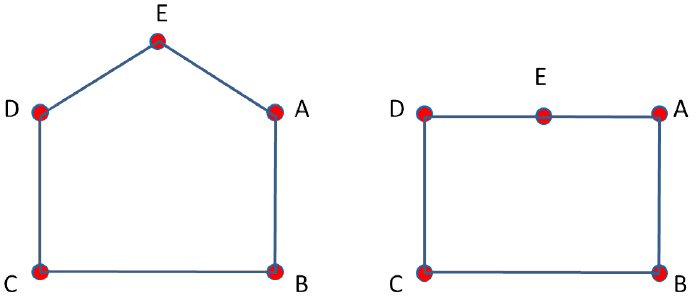
\includegraphics[width=0.7\textwidth]{images/pentagon_verts.png}
		\vfill
	\end{figure}
\end{frame}
%---------------------------
\begin{frame}[t]\frametitle{Vertices A \& E}
    \begin{figure}[t]
		\centering
		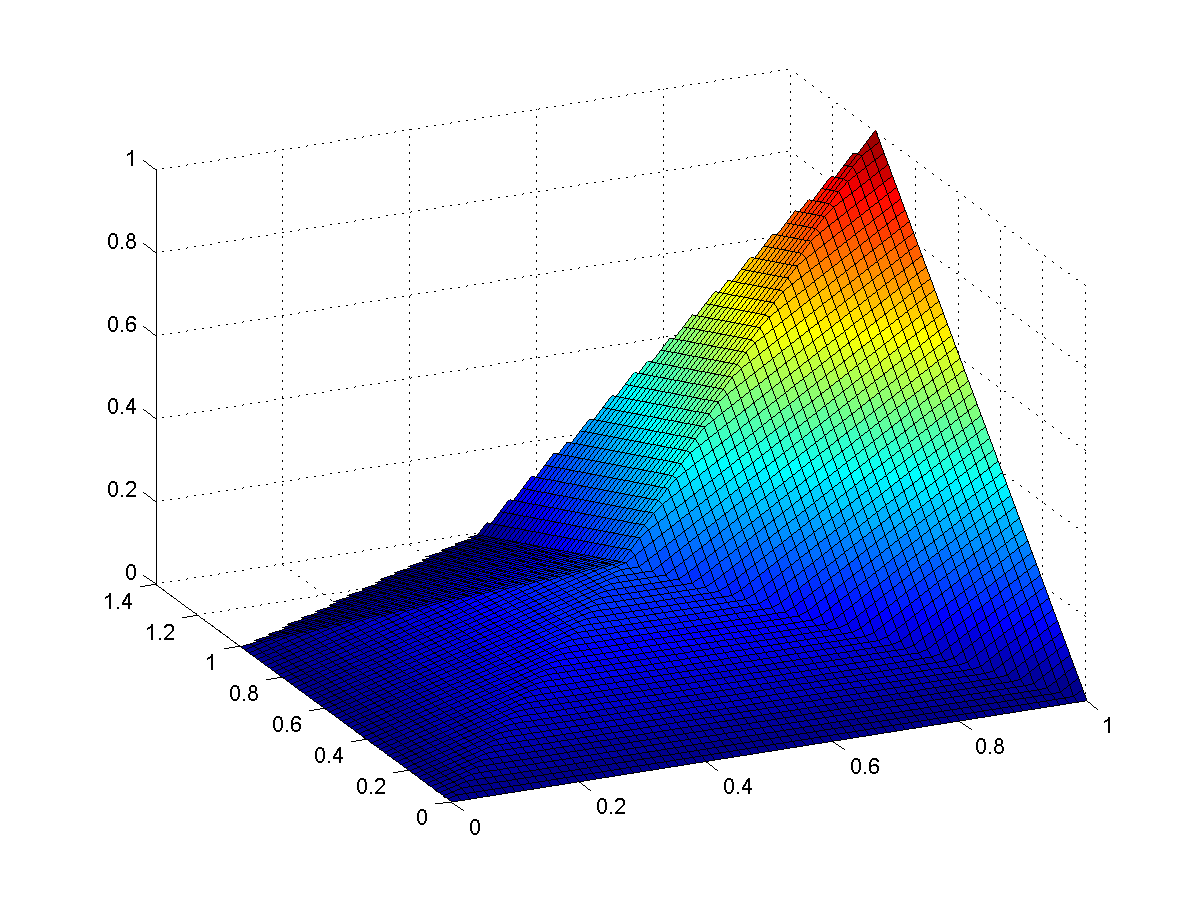
\includegraphics[width=0.38\textwidth]{matlab/pentagon_plot_2_3.png} \hfill
		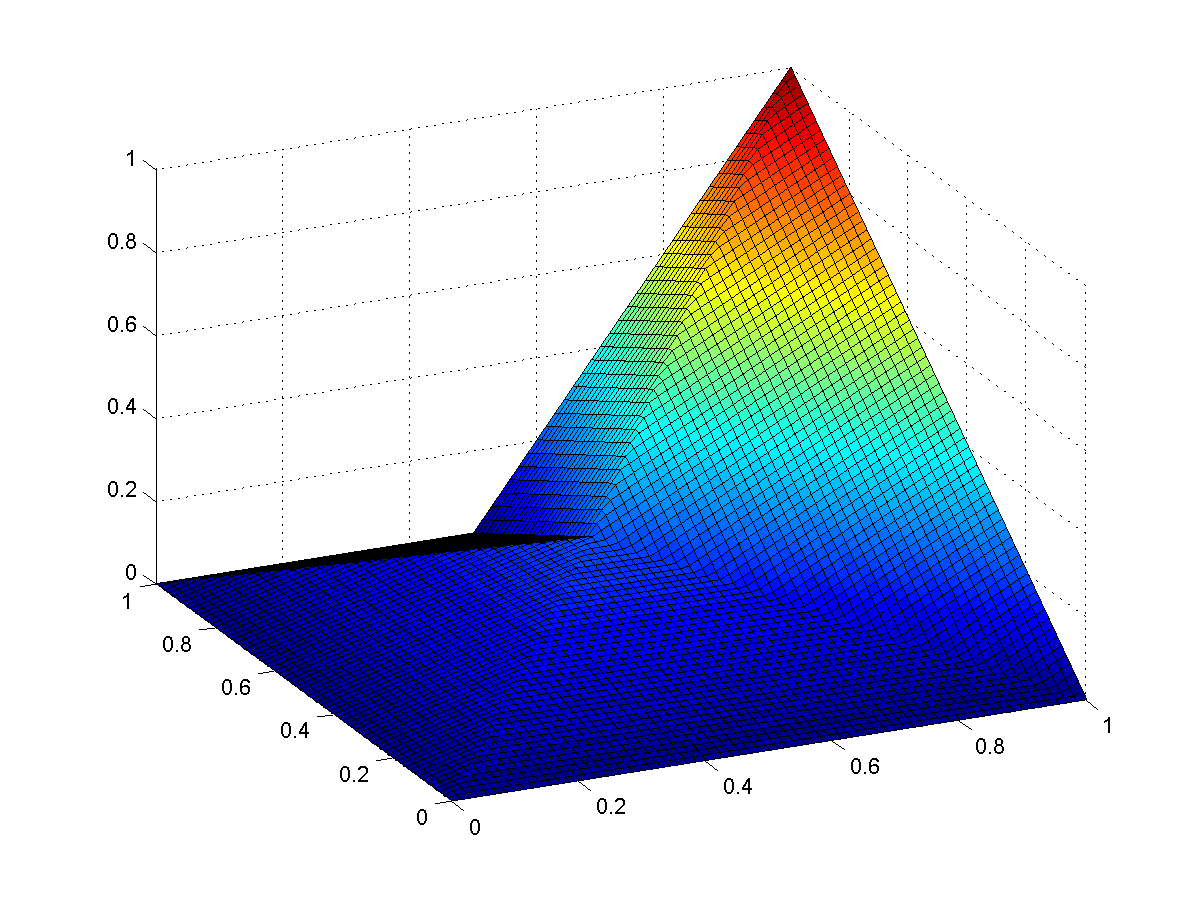
\includegraphics[width=0.38\textwidth]{matlab/d_pentagon_plot_1_3.png} \\ 
		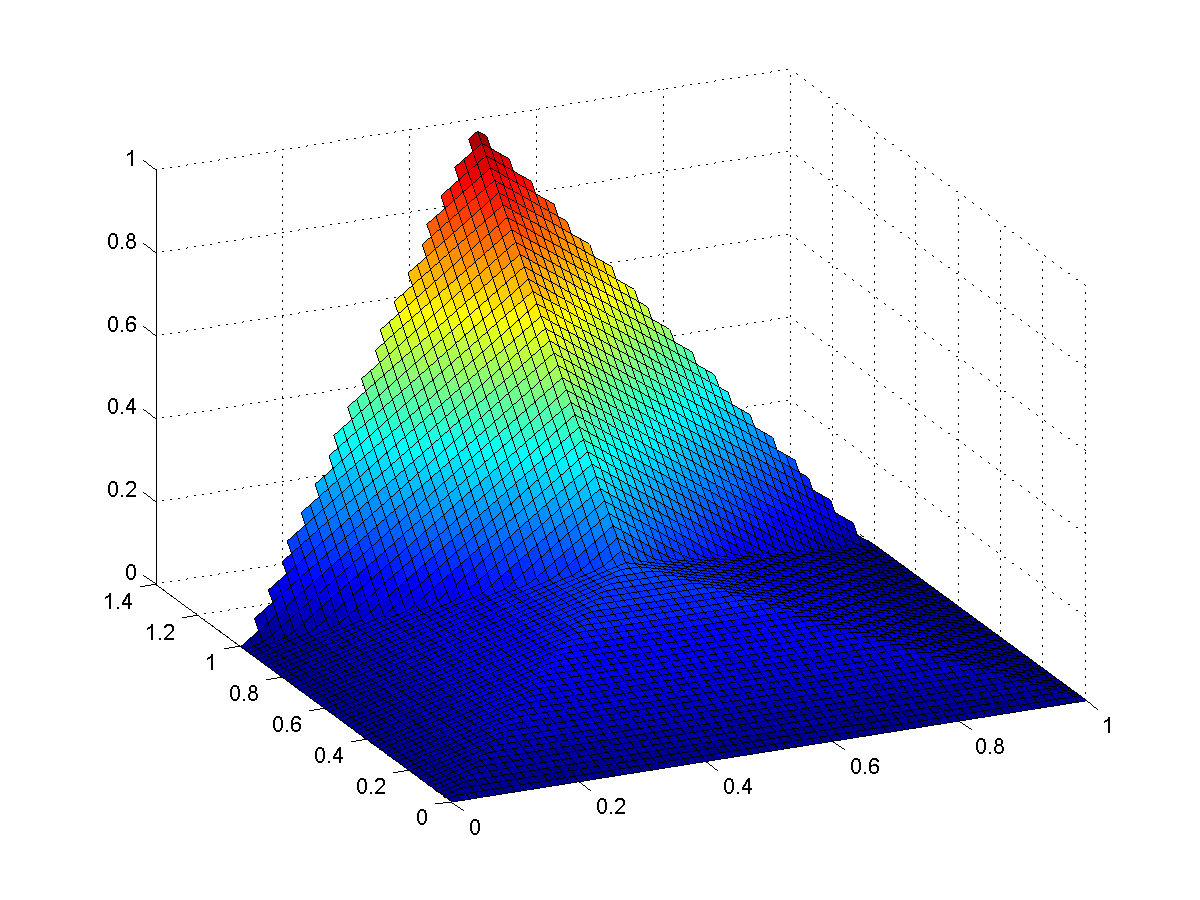
\includegraphics[width=0.38\textwidth]{matlab/pentagon_plot_2_4.png} \hfill
		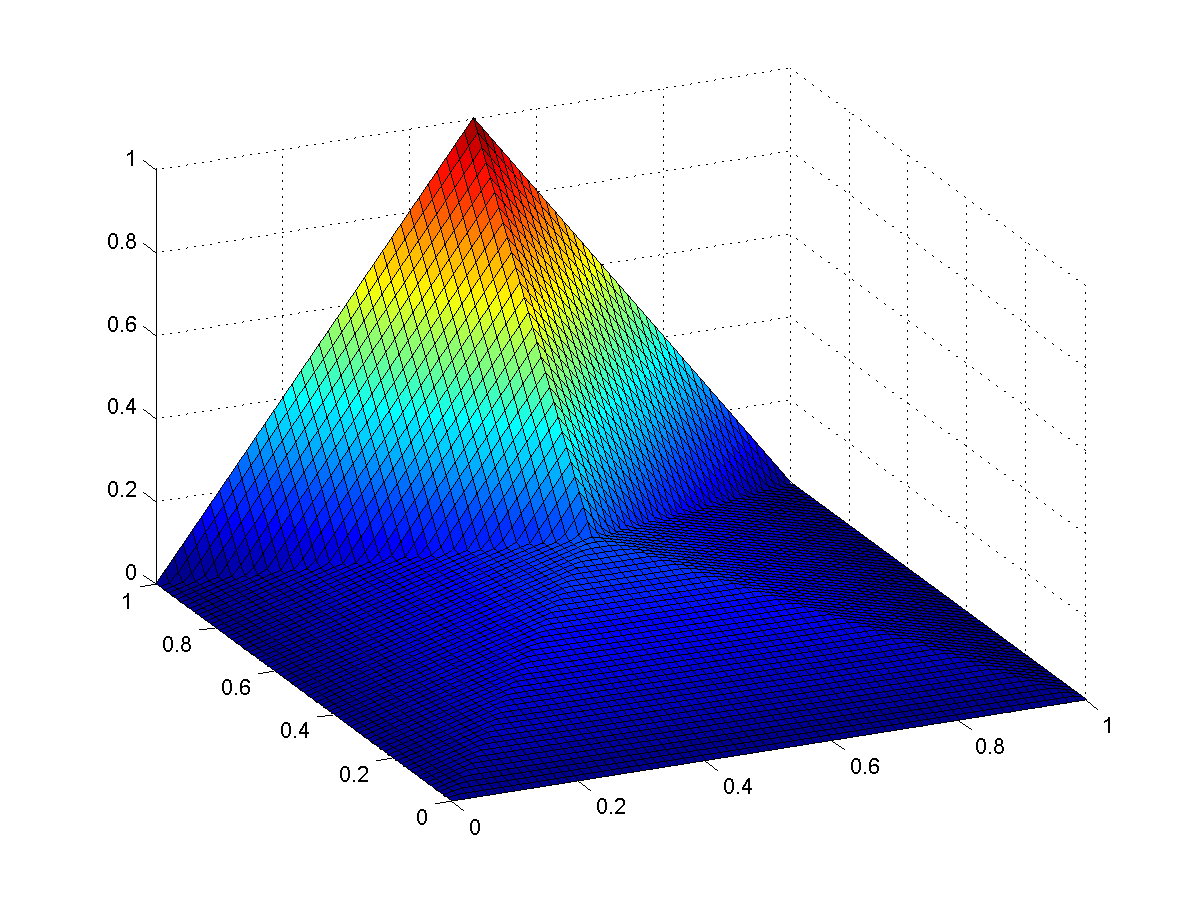
\includegraphics[width=0.38\textwidth]{matlab/d_pentagon_plot_1_4.png}
	\end{figure}
\end{frame}
%---------------------------
%\begin{frame}[t]\frametitle{Vertex A}
 %   \begin{figure}[t]
%		\centering
%		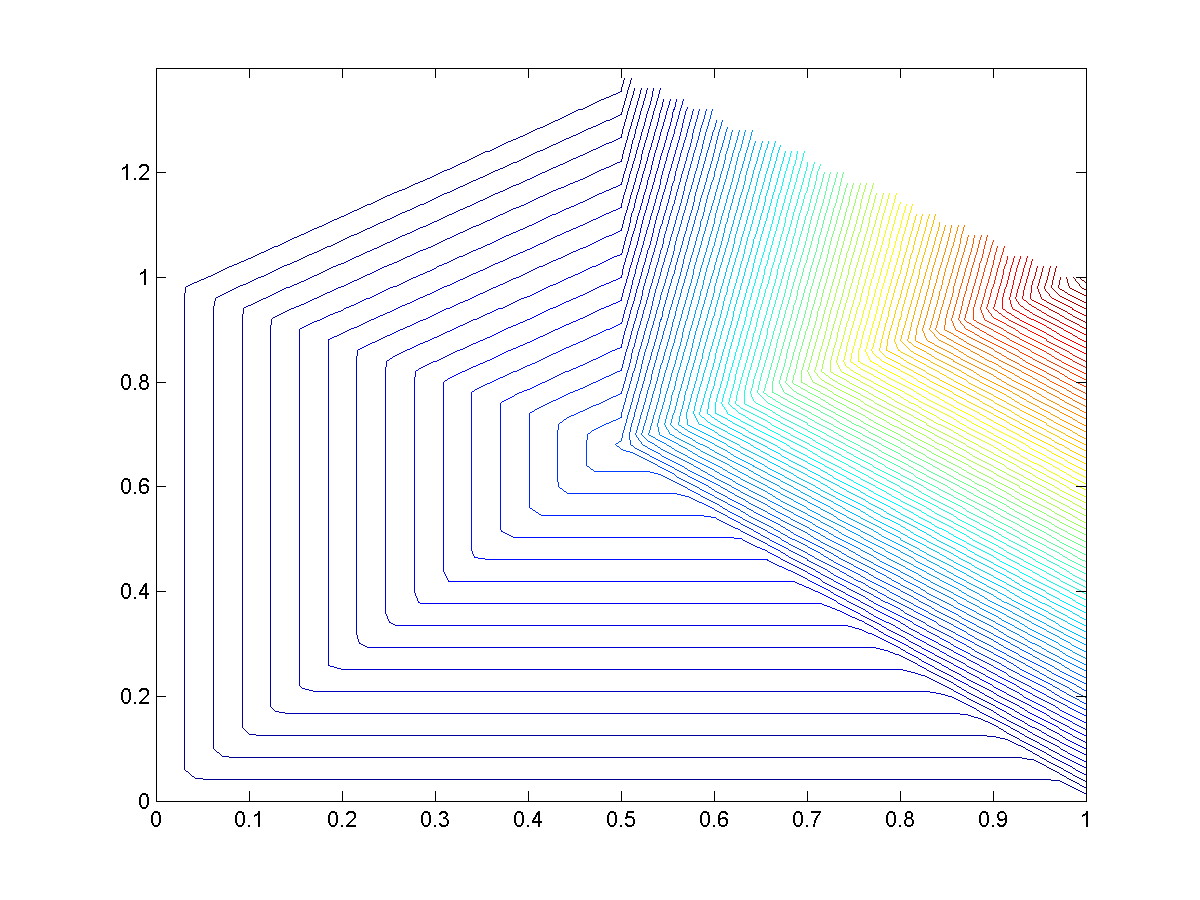
\includegraphics[width=0.38\textwidth]{matlab/pentagon_contour_2_3.png} \hfill
%		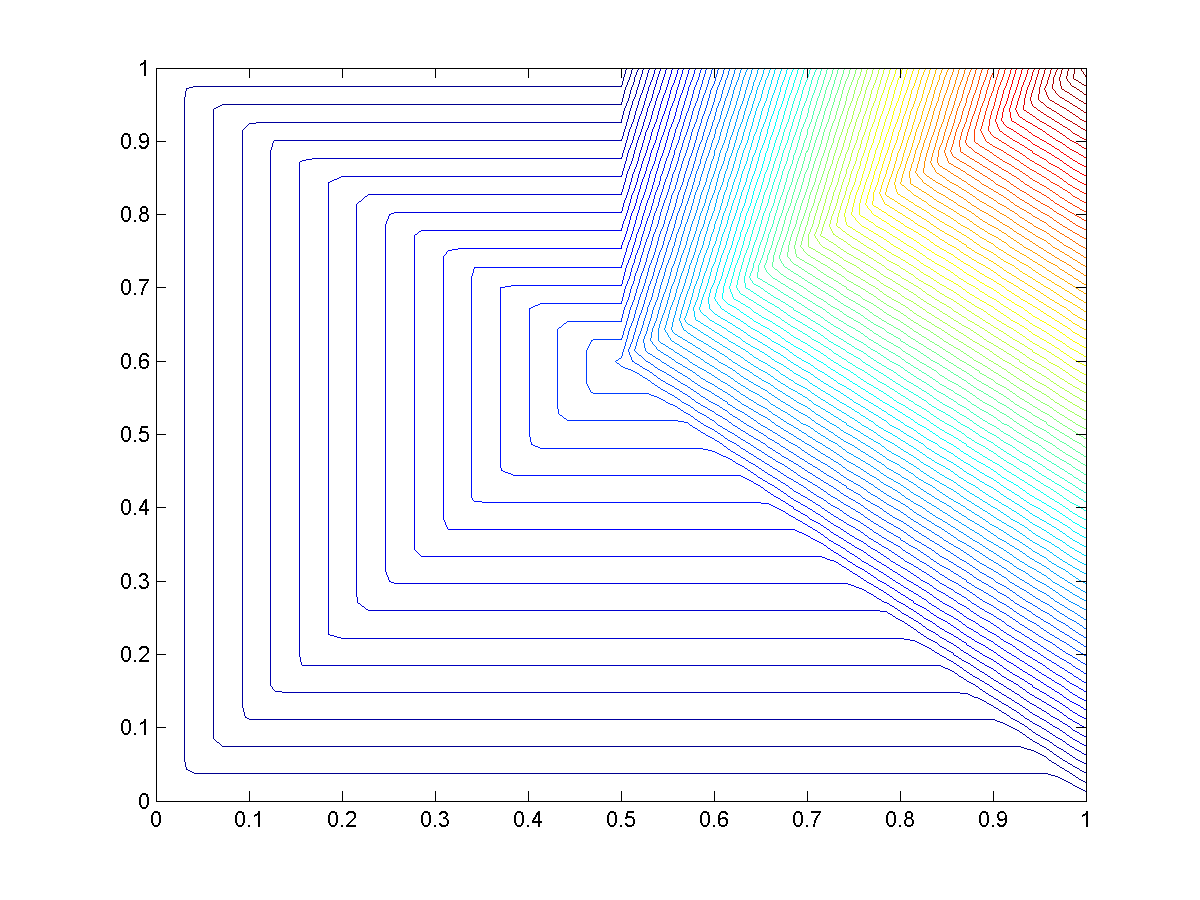
\includegraphics[width=0.38\textwidth]{matlab/d_pentagon_contour_1_3.png} \\
%		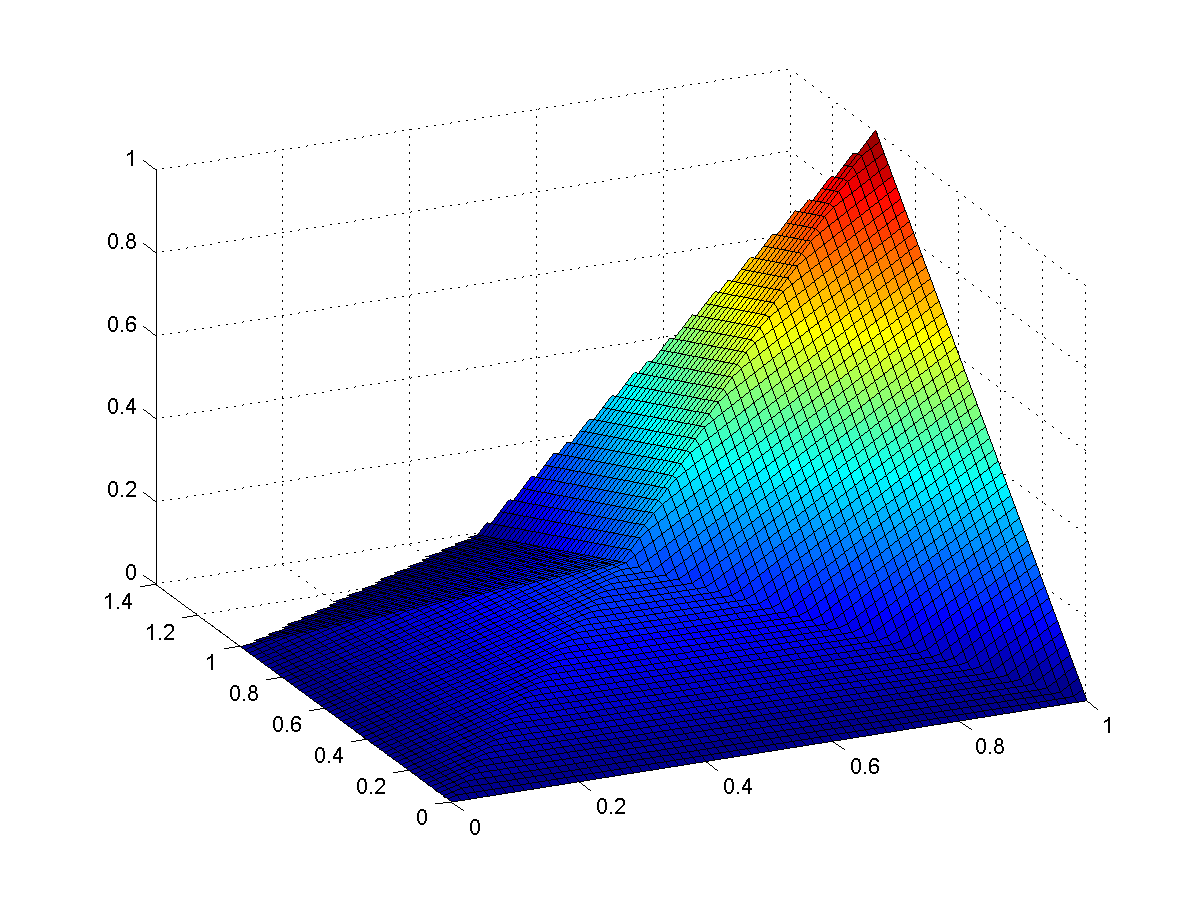
\includegraphics[width=0.38\textwidth]{matlab/pentagon_plot_2_3.png} \hfill
%		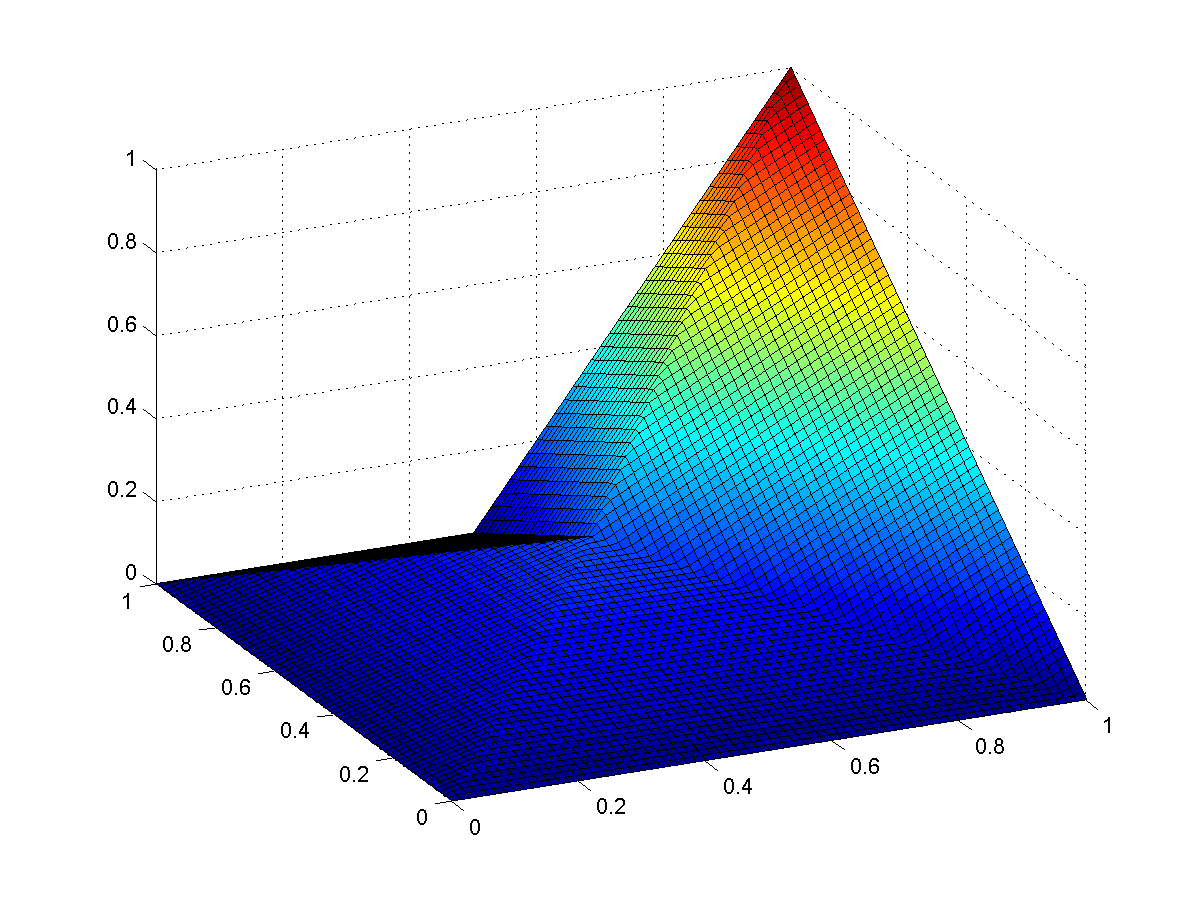
\includegraphics[width=0.38\textwidth]{matlab/d_pentagon_plot_1_3.png}
%	\end{figure}
%\end{frame}
%---------------------------
%\begin{frame}[t]\frametitle{Vertex E}
 %   \begin{figure}[t]
%		\centering
%		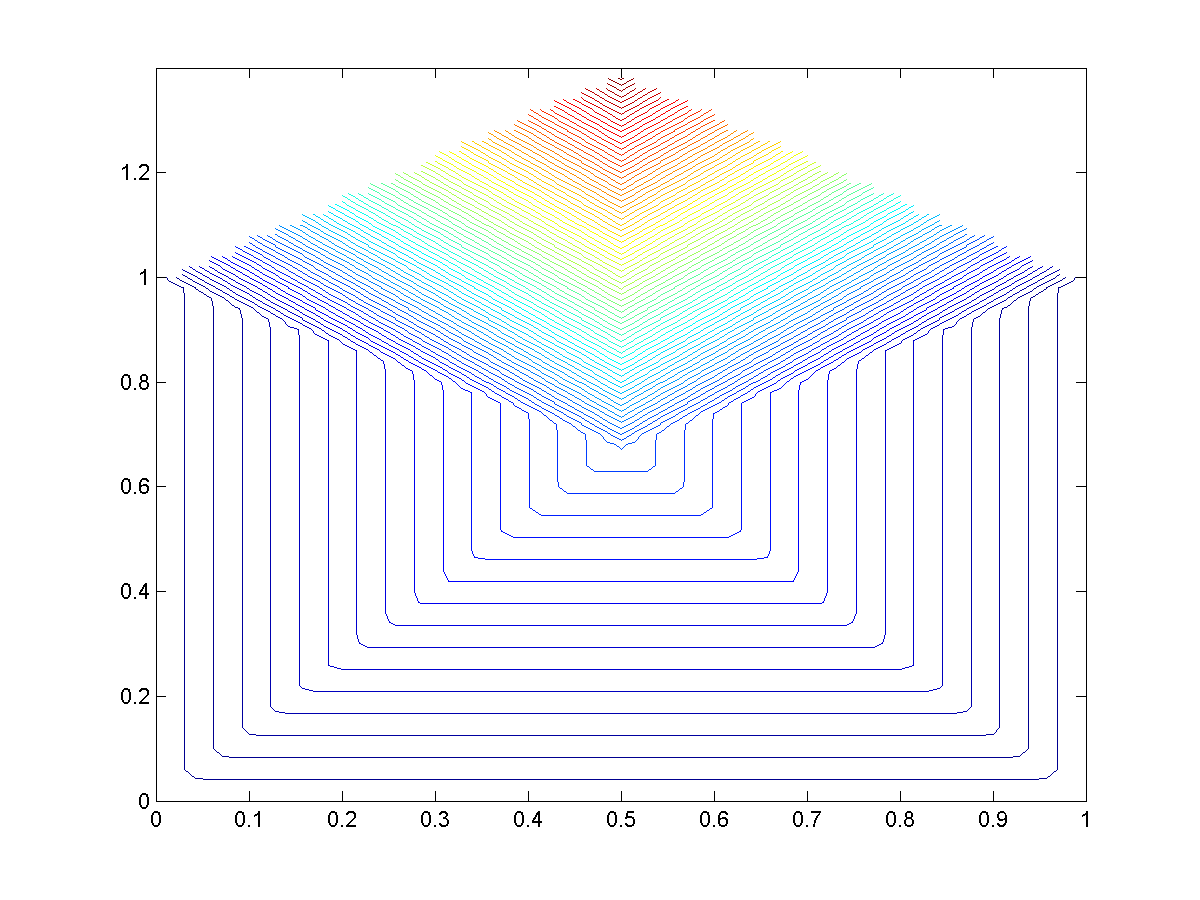
\includegraphics[width=0.38\textwidth]{matlab/pentagon_contour_2_4.png} \hfill
%		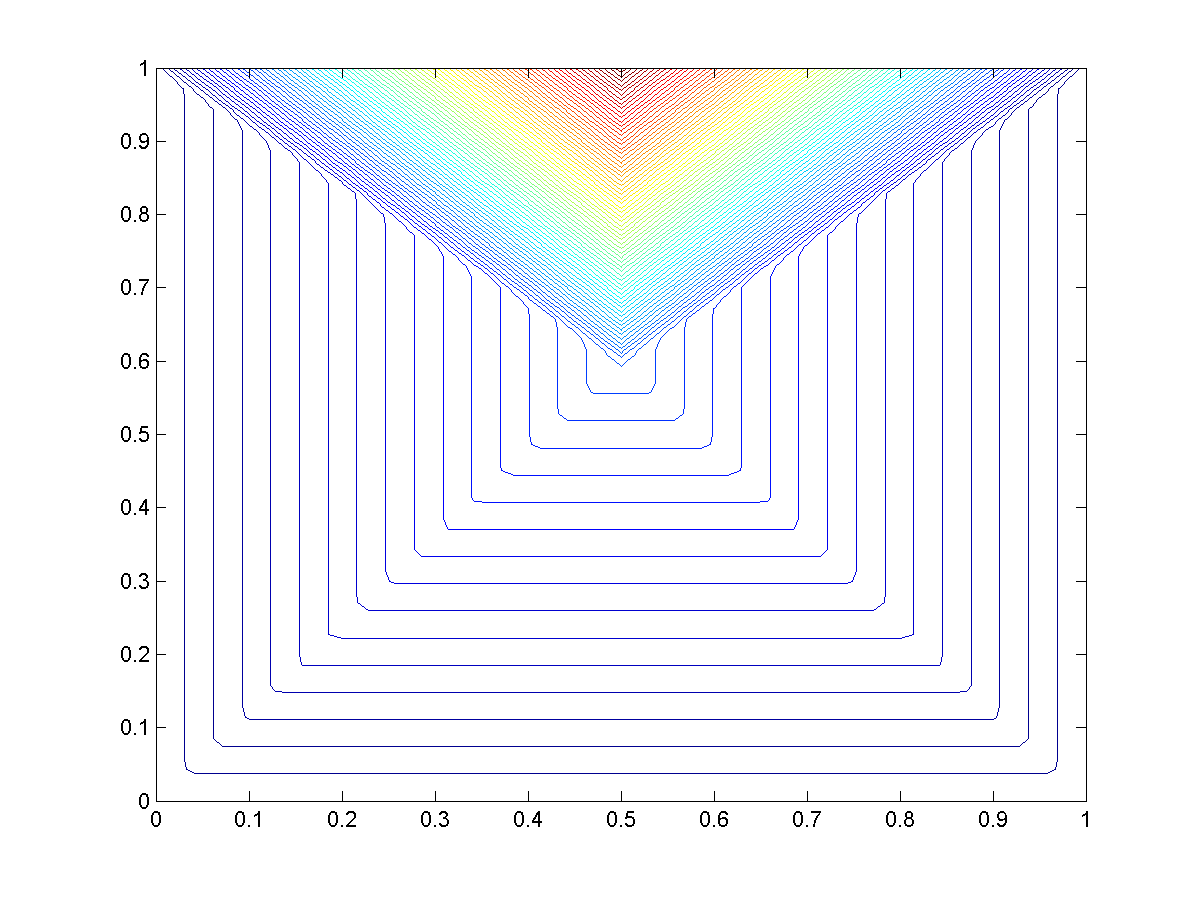
\includegraphics[width=0.38\textwidth]{matlab/d_pentagon_contour_1_4.png} \\
%		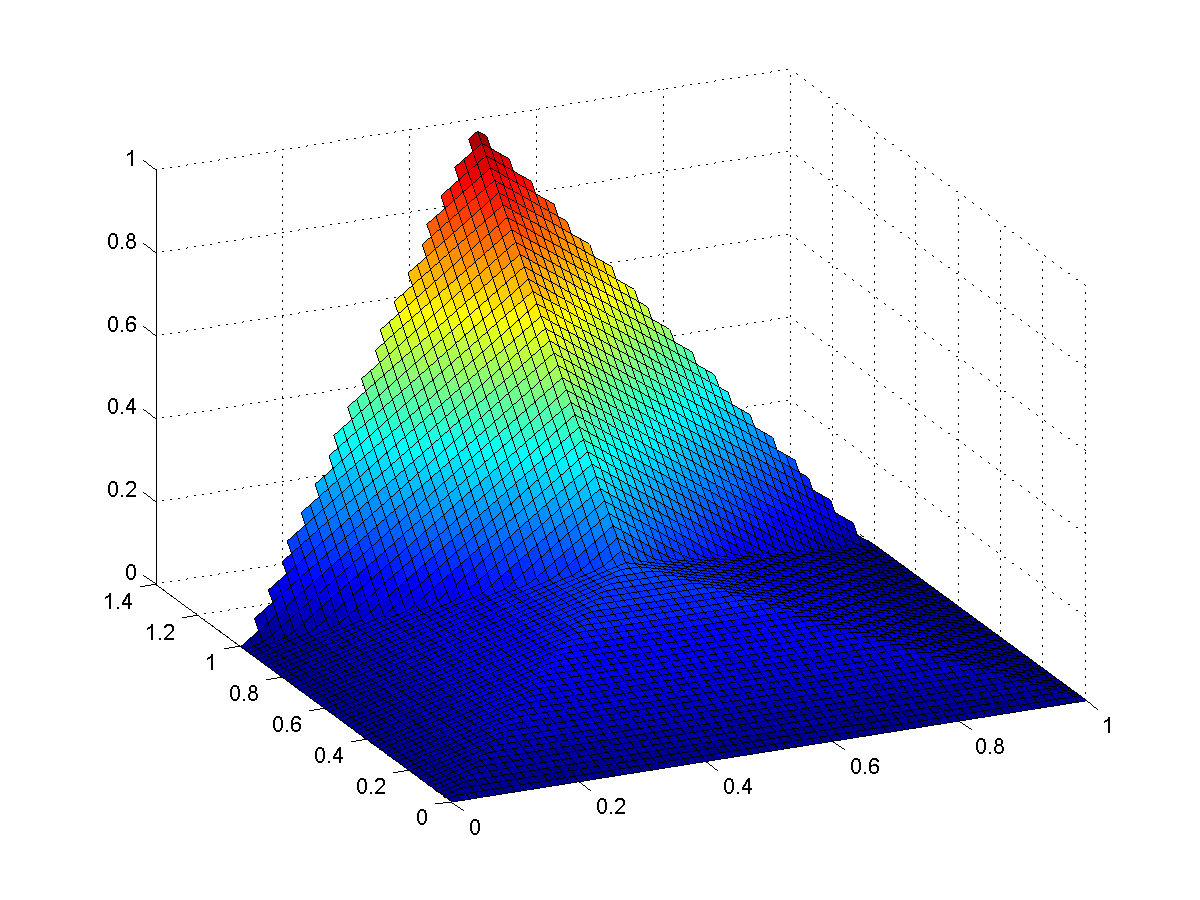
\includegraphics[width=0.38\textwidth]{matlab/pentagon_plot_2_4.png} \hfill
%		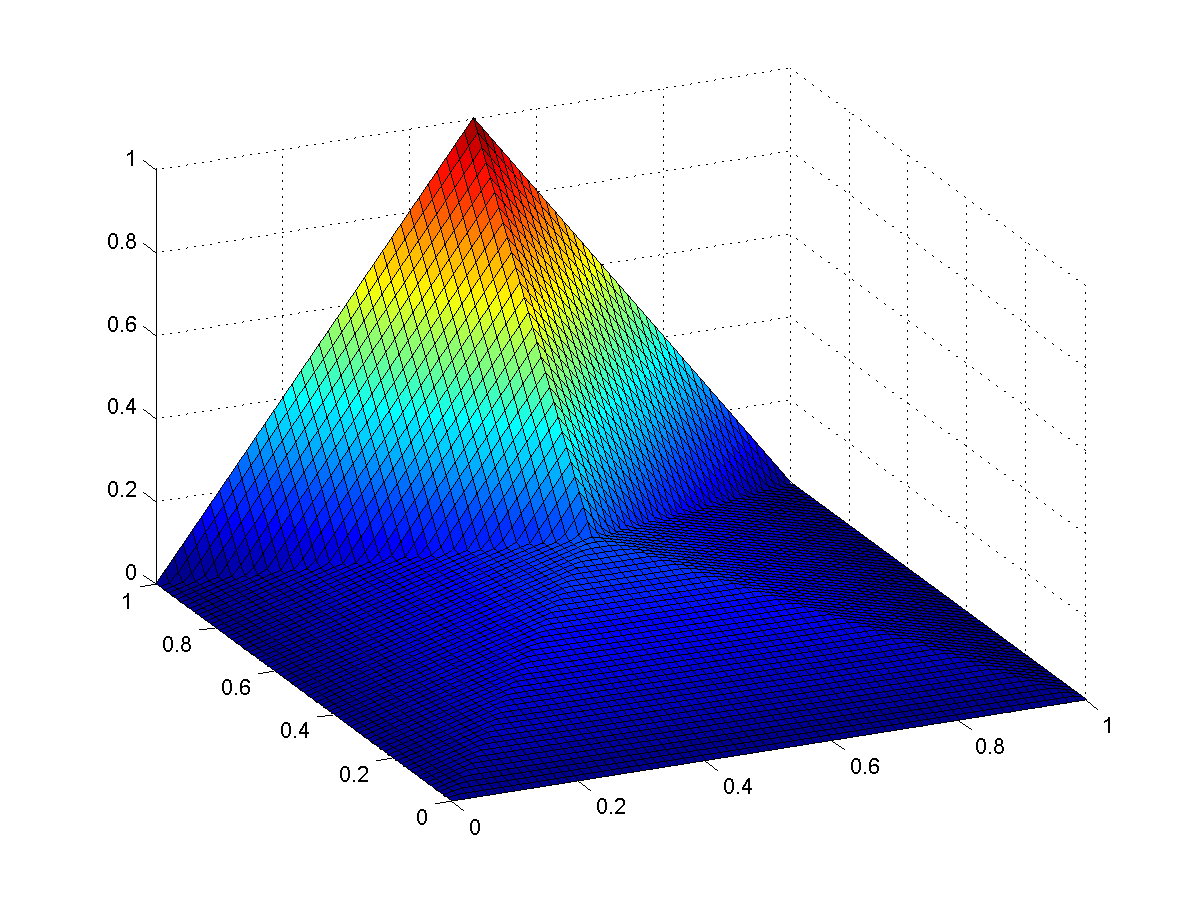
\includegraphics[width=0.38\textwidth]{matlab/d_pentagon_plot_1_4.png}
%	\end{figure}
%\end{frame}
%---------------------------
%\begin{frame}[t]\frametitle{3D PWL - Unit Cube}
%Working on getting this presentable in VisIt.
%\end{frame}
%---------------------------
%%%%%%%%%%%%%%%%%%%%%%%%%%%%%%%%%%%%%%%%%%%%%%%%%%%%%%%%%%%%%
%%%%%%%%%%%%%%%%%%%%%%%%%%%%%%%%%%%%%%%%%%%%%%%%%%%%%%%%%%%%%
\section{Numerical Results}
\subsection{}
%---------------------------
\begin{frame}[t]\frametitle{Numerical Results}
    	\begin{block}{Geometry Specifications}
		\begin{itemize}
			\item Extruded 2D meshes to form 3D prisms
			\item 2D Mesh Types: rectangular, triangles, rand-poly, sine-poly, z-poly
		\end{itemize}
	\end{block}
	\begin{block}{Test Problems}
		\begin{itemize}
			\item Purely-Linear Solution
			\item Method of Manufactured Solutions (MMS)
		\end{itemize}
	\end{block}
\end{frame}
%---------------------------
\begin{frame}[t]\frametitle{Investigated Mesh Types}
	\begin{figure}[t]
		\centering
		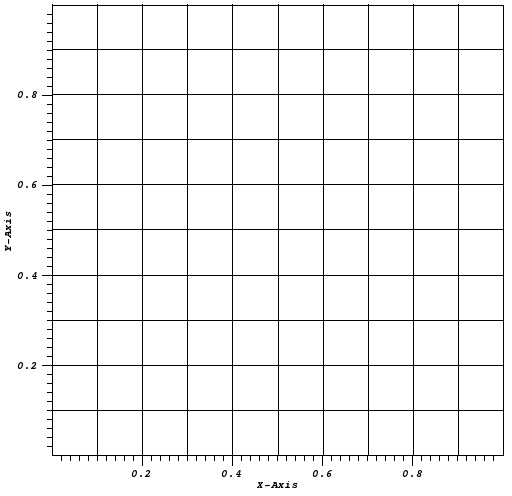
\includegraphics[width=.28\textwidth]{images/cart_mesh.jpg}
		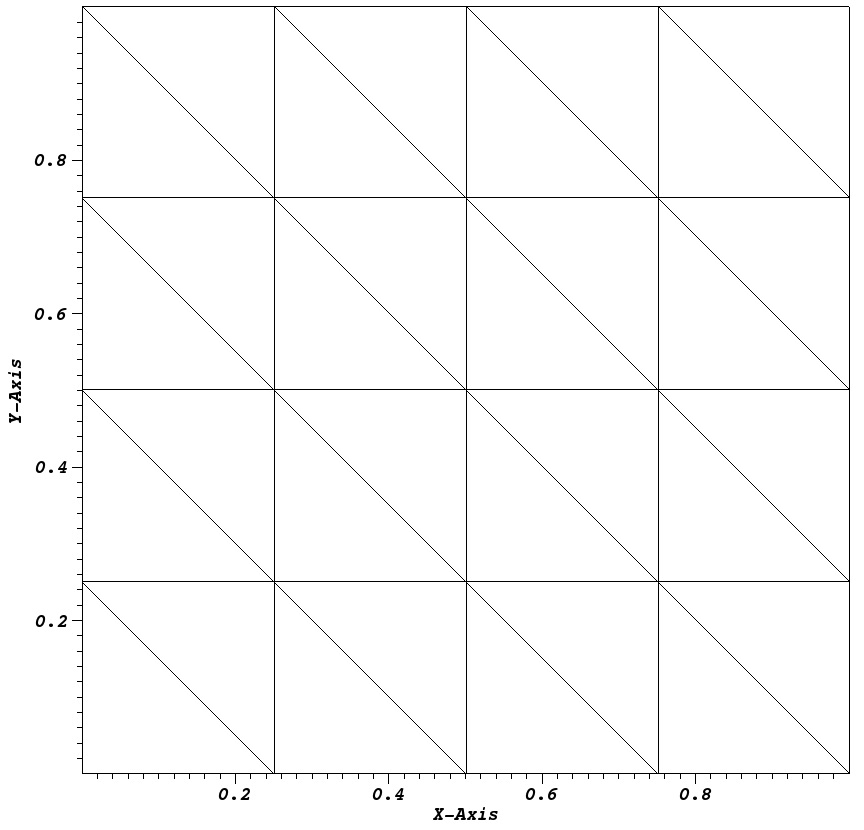
\includegraphics[width=.28\textwidth]{images/tri_mesh.jpg}
		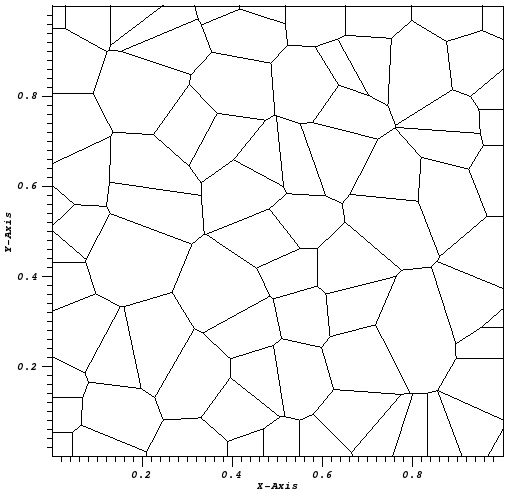
\includegraphics[width=.28\textwidth]{images/poly_mesh.jpg} \\
		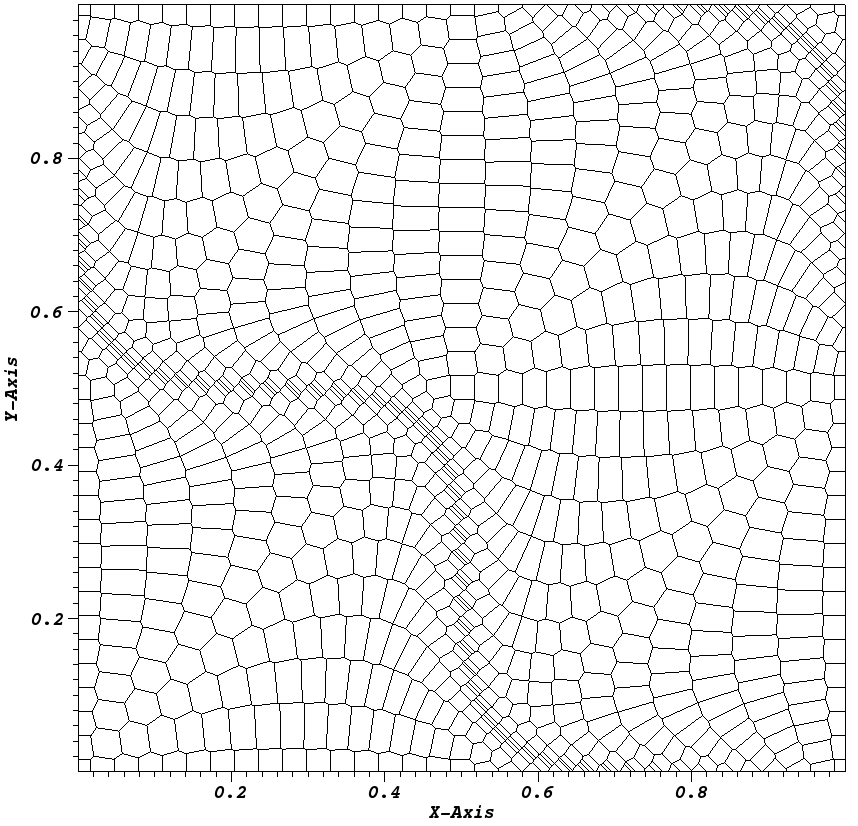
\includegraphics[width=.28\textwidth]{images/sine_poly_mesh.png}
		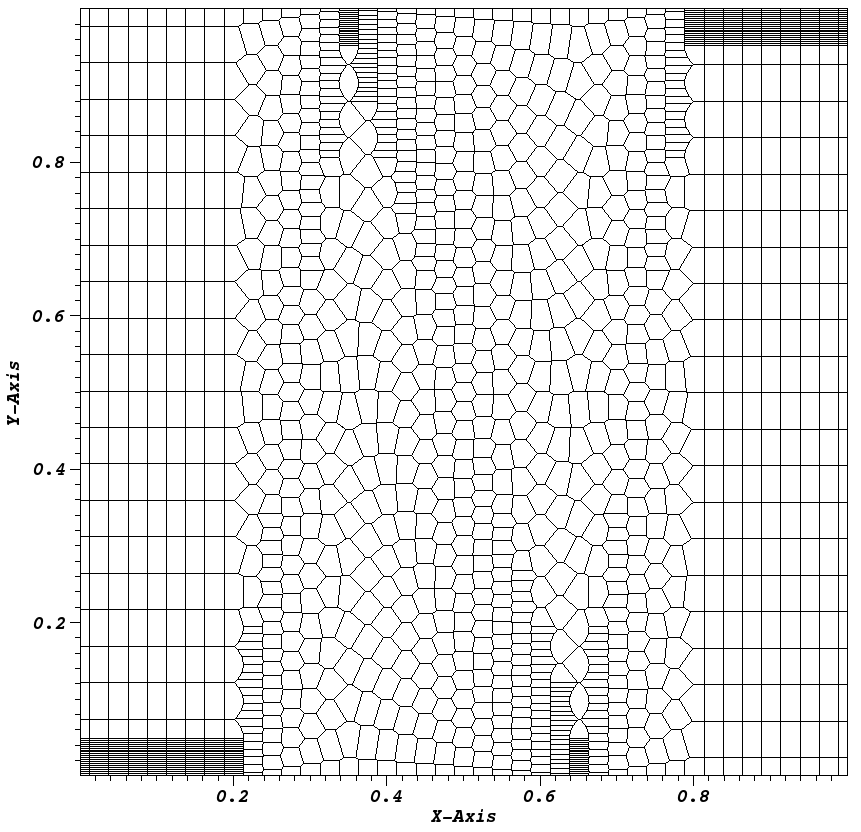
\includegraphics[width=.28\textwidth]{images/z_poly_mesh.png}
	\end{figure}
\end{frame}
%---------------------------
\begin{frame}[t]\frametitle{Linear Solution Test Problems}
    	\begin{block}{Problem Description}
		\begin{itemize}
			\item $\sigma = q = 0$
			\item Robin conditions on 1 set of opposing boundaries; homogeneous Neumann on all others
			\begin{itemize}
				\item Robin conditions on non-axial boundaries
			\end{itemize}
			\item $x,y,z \in (0,L)$
			\item $\Phi (x,y,z) =\frac{4 J^{inc}}{L+4D} \left(  L + 2D - y  \right)$
			\begin{itemize}
				\item $\Phi(0) - 2D \partial_y \Phi|_0 = 4 J^{inc}, \qquad \forall x\text{ at y=0}$
				\item $\Phi(L) + 2D \partial_y \Phi |_L = 0, \qquad \,\,\,\,\,\,\,\,\, \forall x\text{ at y=L} $
			\end{itemize}
		\end{itemize}
	\end{block}
%	\begin{block}{Geometry Description}
%		\begin{itemize}
%			\item Tested all 5 geometry types
%			\item 4 equally-spaced axial extrusion levels
%		\end{itemize}
%		\begin{gather*}
%			 x\in (0,1), \qquad y\in (0,1), \qquad z\in (0,1)
%       	\end{gather*}
%	\end{block}
%\end{frame}
\end{frame}
%---------------------------
\begin{frame}[t]\frametitle{Linear Solution Results}
    	\begin{columns}
		\begin{column}{.5\textwidth}
			\begin{figure}[t]
				\centering
				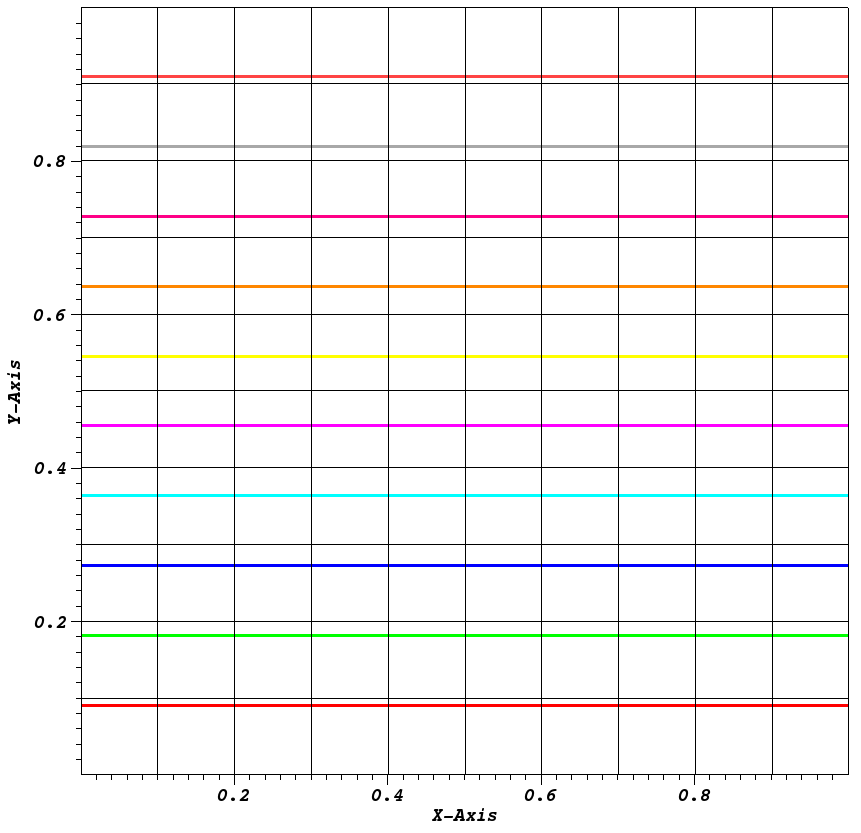
\includegraphics[width=.9\textwidth]{images/cart_lin_contour.png}
			\end{figure}
		\end{column}
		\begin{column}{.5\textwidth}
			\begin{figure}[t]
				\centering
				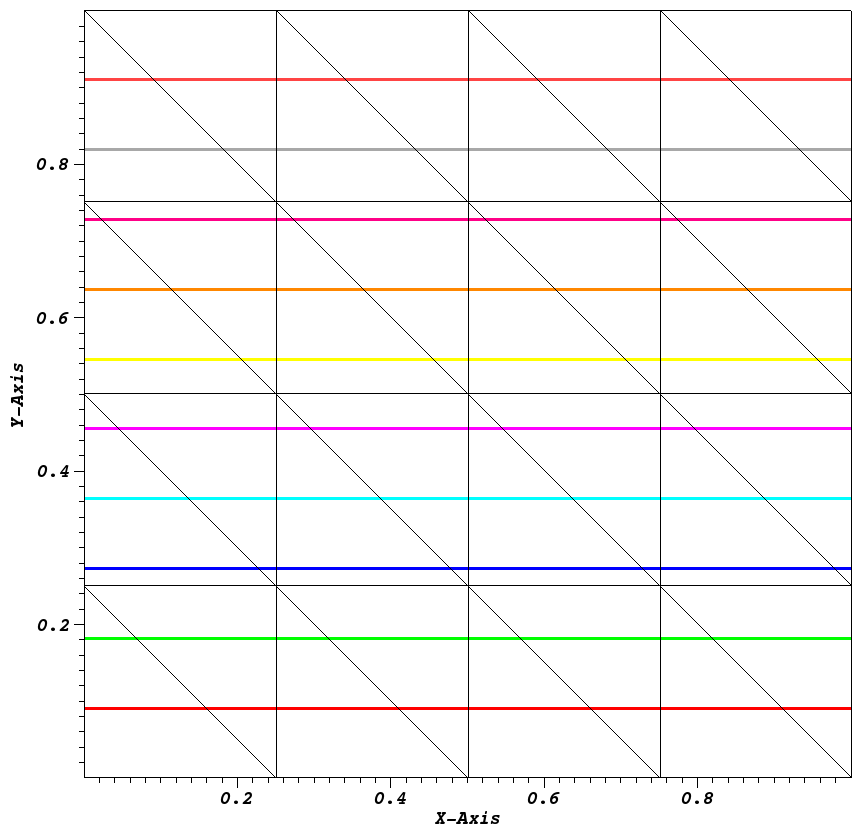
\includegraphics[width=.9\textwidth]{images/tri_lin_contour.png}
			\end{figure}
		\end{column}
	\end{columns}
\end{frame}
%---------------------------
\begin{frame}[t]\frametitle{Linear Solution Results}
    	\begin{columns}
		\begin{column}{.5\textwidth}
			\begin{figure}[t]
				\centering
				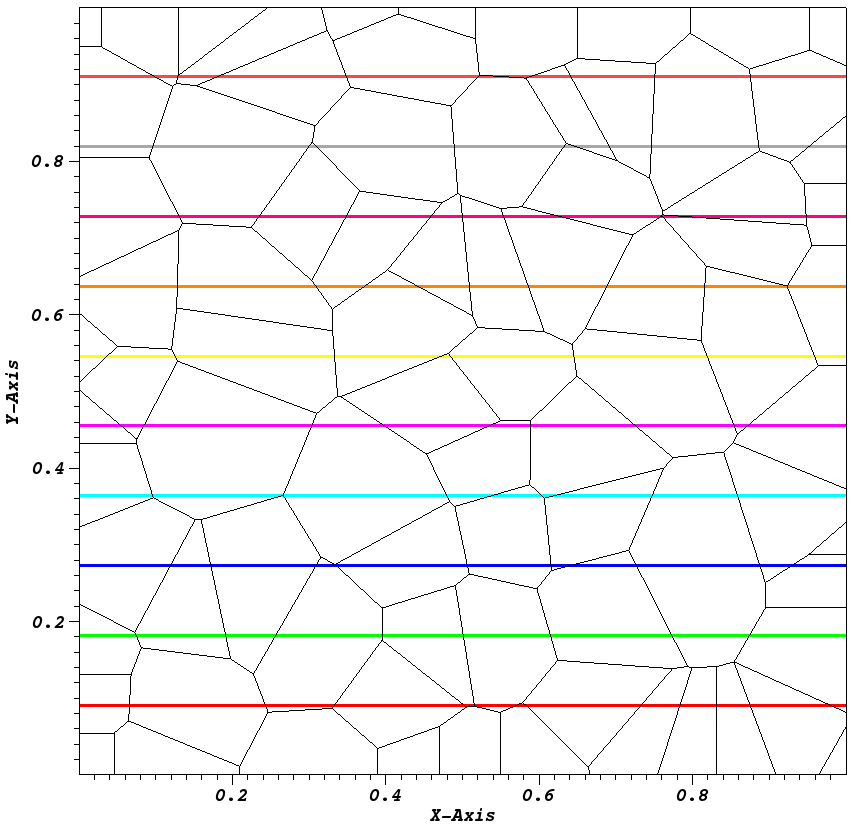
\includegraphics[width=.9\textwidth]{images/poly_lin_contour.png}
			\end{figure}
		\end{column}
		\begin{column}{.5\textwidth}
			\begin{figure}[t]
				\centering
				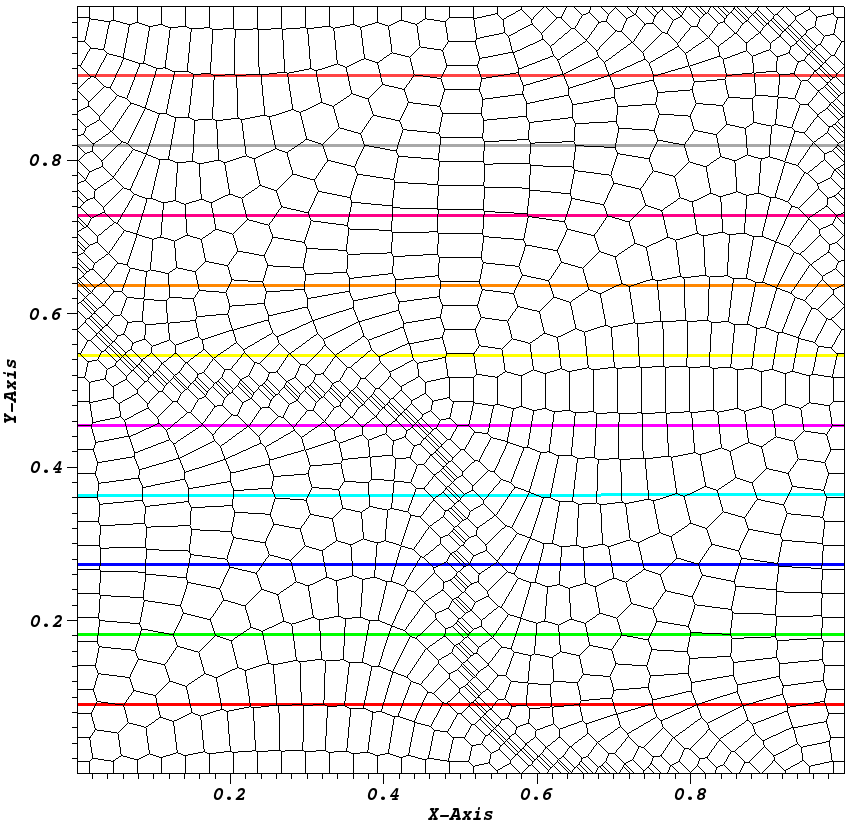
\includegraphics[width=.9\textwidth]{images/sine_poly_lin_contour.png}
			\end{figure}
		\end{column}
	\end{columns}
\end{frame}
%---------------------------
\begin{frame}[t]\frametitle{Linear Solution Results}
	\begin{figure}[t]
		\centering
		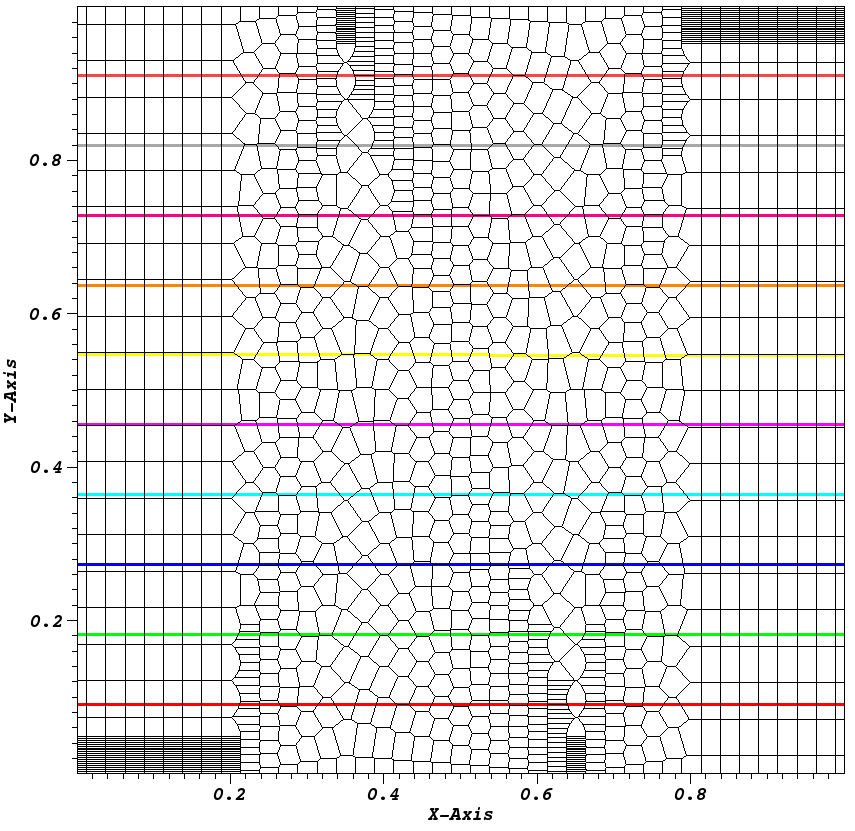
\includegraphics[width=.5\textwidth]{images/z_poly_lin_contour.png}
	\end{figure}
\end{frame}
%---------------------------
\begin{frame}[t]\frametitle{MMS Solutions}
    	\begin{block}{Problem Description}{\small
		\begin{itemize}
			\item Tested 2 solution forms
		\end{itemize}
		\begin{gather*}
			 \Phi_1 (x,y,z) = x(1-x) y (1-y) z (1-z) \\
			 \Phi_2 (x,y,z) = \Phi_1 (x,y,z) \exp(-\left(  (x-x_0)^2 + (y-y_0)^2 + (z-z_0)^2 \right)) \\ 
			x\in (0,1), \qquad y\in (0,1), \qquad z\in (0,1), \qquad  x_0=y_0=z_0=3/4
        	\end{gather*}
		\begin{itemize}
			\item Compared SIP to CFEM solutions also using PWL basis functions
			\item Tested \# of unknowns, $N$: $ O( 10^1) - O(10^5)$
			\item Order of Convergence in 3D: $|| u - u_h ||_{L^2} \propto N^{-2/3}$
			\begin{itemize}
				\item $|| u - u_h ||_{L^2} \propto h^2, \qquad h \propto N^{- \text{dim}}$
			\end{itemize}
		\end{itemize}}
	\end{block}
\end{frame}
%---------------------------
\begin{frame}[t]\frametitle{MMS Solutions - $\Phi_1 (x,y,z)$}
    	\begin{figure}[t]
		\centering
		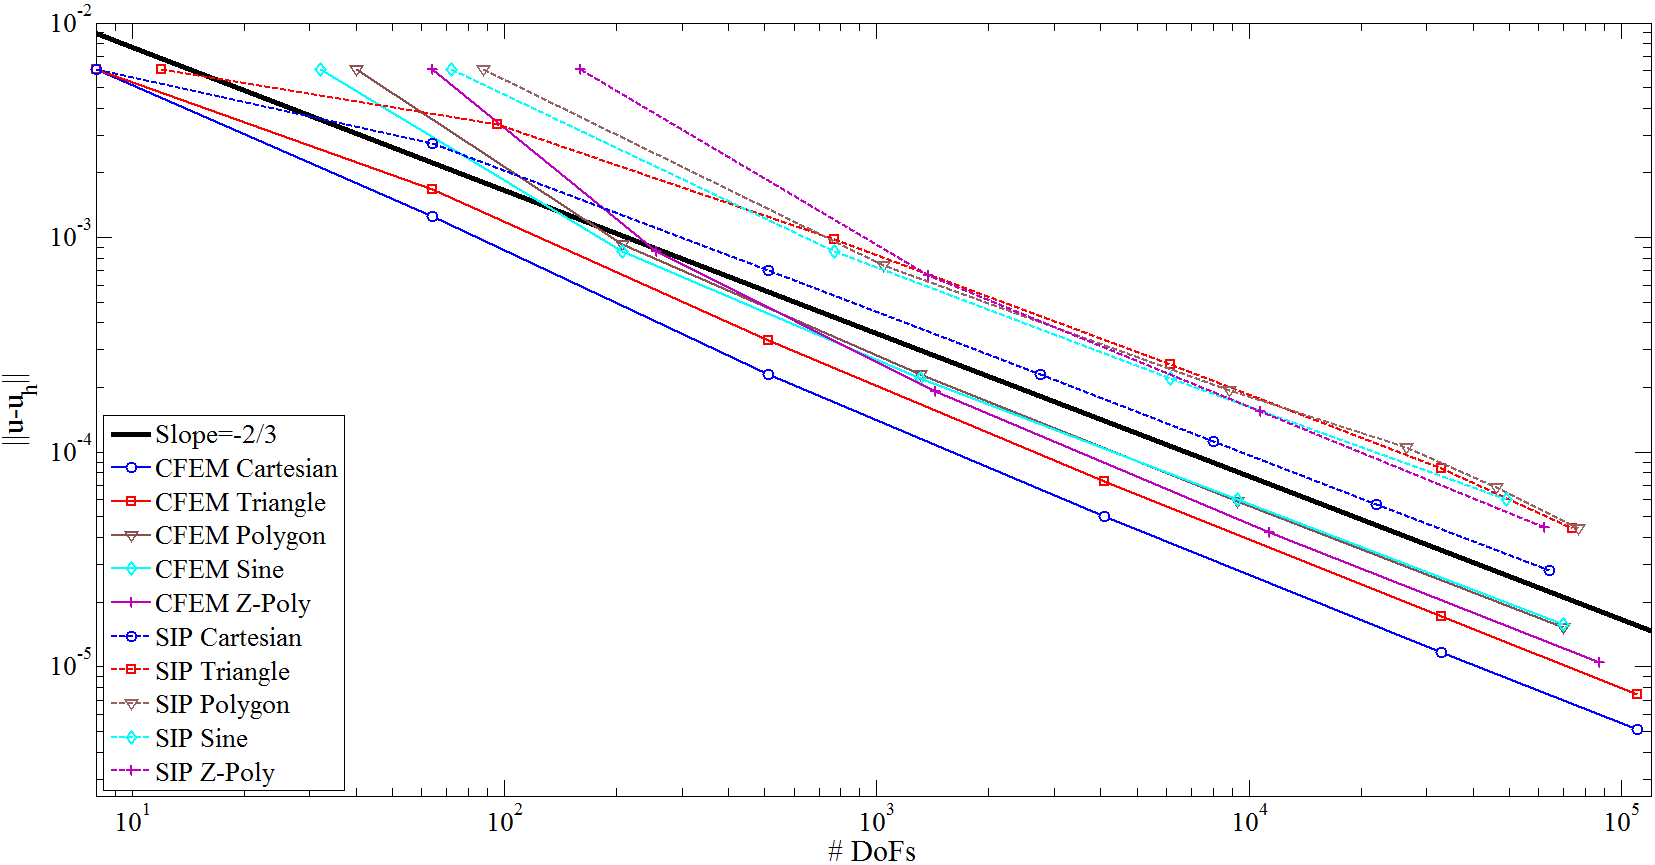
\includegraphics[width=1.0\textwidth]{images/mms_3d_quad_full_paint.png}
	\end{figure}
\end{frame}
%---------------------------
\begin{frame}[t]\frametitle{MMS Solutions - $\Phi_2 (x,y,z)$}
    	\begin{figure}[t]
		\centering
		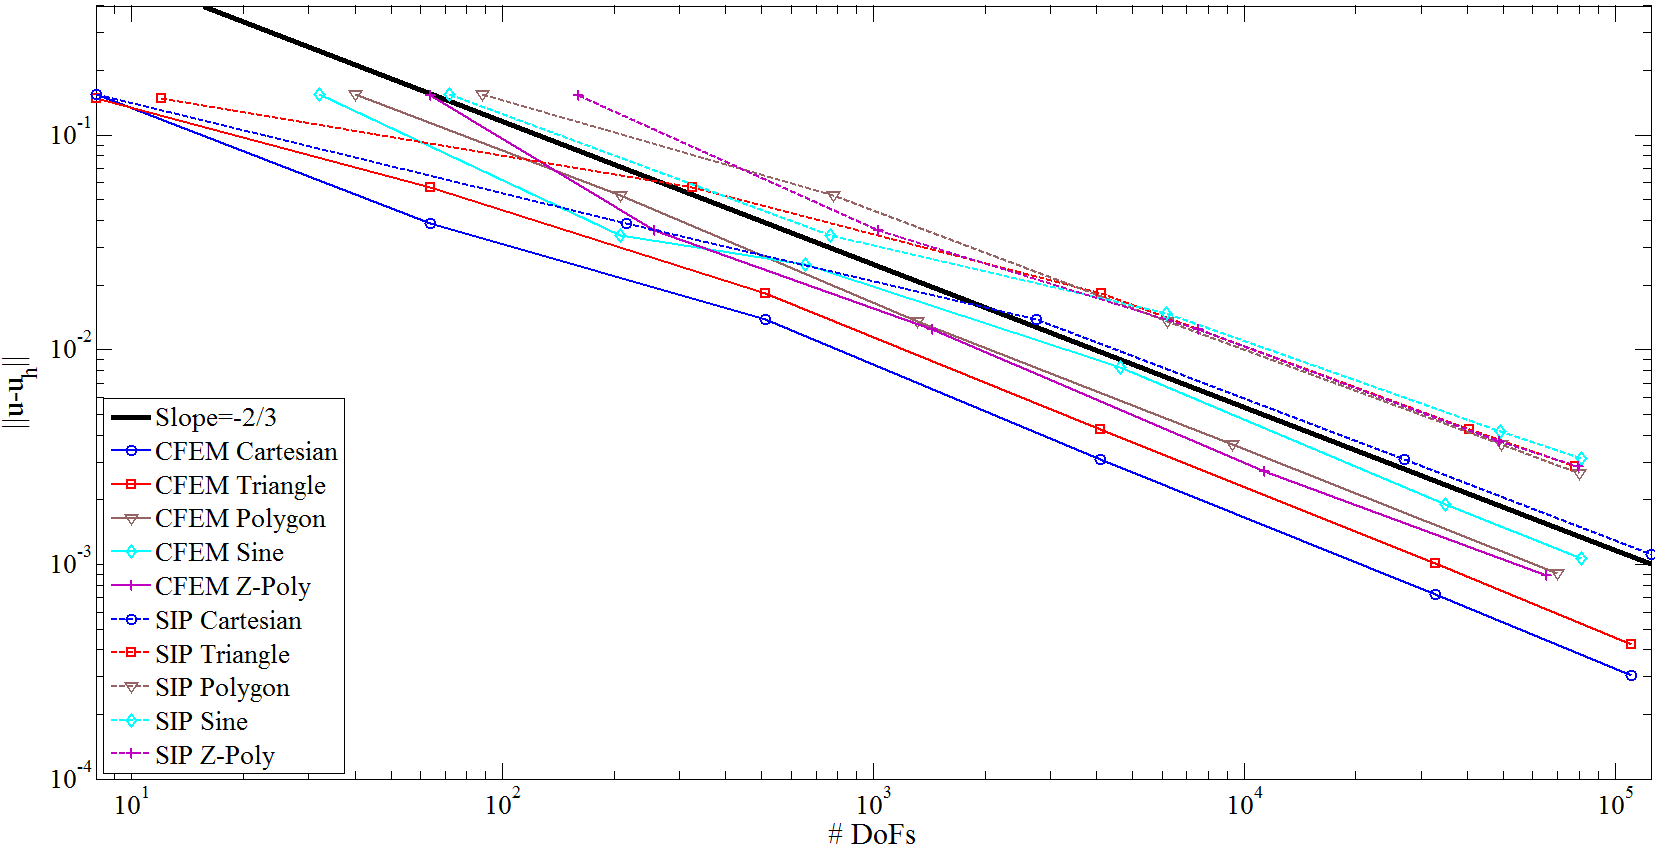
\includegraphics[width=1.0\textwidth]{images/mms_3d_gauss_full_paint.png}
	\end{figure}
\end{frame}
%---------------------------
%%%%%%%%%%%%%%%%%%%%%%%%%%%%%%%%%%%%%%%%%%%%%%%%%%%%%%%%%%%%%
%%%%%%%%%%%%%%%%%%%%%%%%%%%%%%%%%%%%%%%%%%%%%%%%%%%%%%%%%%%%%
\section{Conclusions}
\subsection{}
%---------------------------
\begin{frame}[t]\frametitle{Conclusions and Future Work}
	\begin{block}{Conclusions}
		\begin{itemize}
			\item Tested a 3D extension of the SIP DFEM diffusion formulation using PWL basis functions
			\item A purely-linear solution is captured 
			\item Verified second-order convergence on 3D polyhedral grids
		\end{itemize}
	\end{block}
	\begin{block}{Future Work}
		\begin{itemize}
			\item Implementation in PDT as a DSA preconditioner (debug phase)
			\item Integration with HYPRE's AMG numerical solver
		\end{itemize}
	\end{block}
\end{frame}

\end{document}